\documentclass[11pt,letterpaper]{article}
% isms-27000-style.tex
% Suite preamble for the ISO/IEC 27000/27001/27002 ISMS engineering suite.
%
% RECONSTRUCTION PROVENANCE: the ten uploaded suite documents load a shared
% preamble with `\input{style.tex}`, but no `style.tex` was present in the
% upload batches or anywhere in this repository's history. This file is a
% documented, suite-specific reconstruction inferred from the macros, colors
% and environments the documents actually use (colors navy/teal/graytext/pale;
% tag commands \SourceTag, \EngineeringTag, \SourceNote{..}; breakable
% tcolorbox callouts; color-striped longtables; TikZ flow diagrams). It is
% NOT the recovered original style; the original visual design is unknown.
%
% pdfLaTeX only.
\usepackage[T1]{fontenc}
\usepackage[utf8]{inputenc}
\usepackage{lmodern}
\usepackage{microtype}
\usepackage[letterpaper,margin=0.9in,headheight=15pt]{geometry}
\usepackage[table]{xcolor}
\definecolor{navy}{HTML}{14355A}
\definecolor{teal}{HTML}{0A7580}
\definecolor{graytext}{HTML}{55616E}
\definecolor{pale}{HTML}{EFF5F7}
\usepackage{amsmath,amssymb}
\usepackage{array,booktabs,longtable,tabularx,multirow}
\usepackage{enumitem}
\usepackage[most]{tcolorbox}
\usepackage{tikz}
\usetikzlibrary{arrows.meta,positioning,shapes.geometric,fit,calc}
\usepackage{needspace}
\usepackage{titlesec}
\usepackage{fancyhdr}
\usepackage{lastpage}
\usepackage{hyperref}
\hypersetup{colorlinks=true,linkcolor=navy,urlcolor=teal,citecolor=navy,pdfauthor={ISMS Engineering Documentation Suite},pdfsubject={Original supporting guidance for ISO/IEC 27000, 27001 and 27002}}
\setlength{\parindent}{0pt}
\setlength{\parskip}{5pt plus 1pt}
\setlength{\emergencystretch}{2em}
\renewcommand{\arraystretch}{1.18}
\setlist[itemize]{itemsep=2pt,topsep=3pt,leftmargin=1.5em}
\setlist[enumerate]{itemsep=2pt,topsep=3pt,leftmargin=1.7em}
\titleformat{\section}{\Large\bfseries\color{navy}}{\thesection}{0.7em}{}[\vspace{-3pt}\color{teal}\titlerule]
\titleformat{\subsection}{\large\bfseries\color{navy}}{\thesubsection}{0.6em}{}
\titleformat{\subsubsection}{\normalsize\bfseries\color{teal}}{\thesubsubsection}{0.55em}{}
\pagestyle{fancy}
\fancyhf{}
\fancyhead[L]{\sffamily\footnotesize ISO/IEC 27000 series | ISMS Engineering}
\fancyhead[R]{\sffamily\footnotesize\color{graytext} Independent companion}
\fancyfoot[L]{\sffamily\scriptsize Original explanatory material; consult the licensed standards}
\fancyfoot[R]{\sffamily\scriptsize\thepage\ / \pageref{LastPage}}
\renewcommand{\headrulewidth}{0.3pt}
% Inline provenance tags used throughout the suite: \SourceTag marks
% statements grounded in the standards; \EngineeringTag marks original
% engineering interpretation. Both are zero-argument label commands.
\newcommand{\SourceTag}{\textsf{\footnotesize\bfseries\color{navy}[Standard]}~}
\newcommand{\EngineeringTag}{\textsf{\footnotesize\bfseries\color{teal}[Engineering]}~}
\newcommand{\SourceNote}[1]{\par\smallskip{\footnotesize\color{graytext}\textit{Trace: #1.}}\par}

\begin{document}
\pagenumbering{roman}
\begin{titlepage}
\vspace*{1.2in}
{\color{teal}\rule{\textwidth}{4pt}}\par\vspace{20pt}
{\Huge\bfseries\color{navy} Security Architecture and Engineering}\par\vspace{18pt}
{\Large\color{graytext} Reference architecture, design decisions, layered controls and verification criteria}\par\vspace{1.3in}
{\large ISO/IEC 27000:2018 $\vert$ ISO/IEC 27001:2022 $\vert$ ISO/IEC 27002:2022}\par
\vfill
\textbf{Independent educational and engineering implementation reference}\par
Version 1.0 $\cdot$ October 2026\par
{\small Original explanatory material. Source standards are copyrighted; consult licensed originals for authoritative requirements.}\par
\end{titlepage}
\tableofcontents\clearpage\pagenumbering{arabic}
\section{Design assumptions and viewpoints}
\begin{itemize}
\item Business viewpoint: customer obligations, objectives, material risks and accountable decisions.
\item Information viewpoint: classifications, flows, processing geographies, integrity and retention.
\item Application viewpoint: trust boundaries, identities, dependencies and data paths.
\item Technology viewpoint: endpoint, network, runtime, cloud, facility and telemetry layers.
\item Assurance viewpoint: testability, evidence lineage, control operation and management review.
\end{itemize}

\section{Reference security/assurance architecture}
\begin{center}\resizebox{\textwidth}{!}{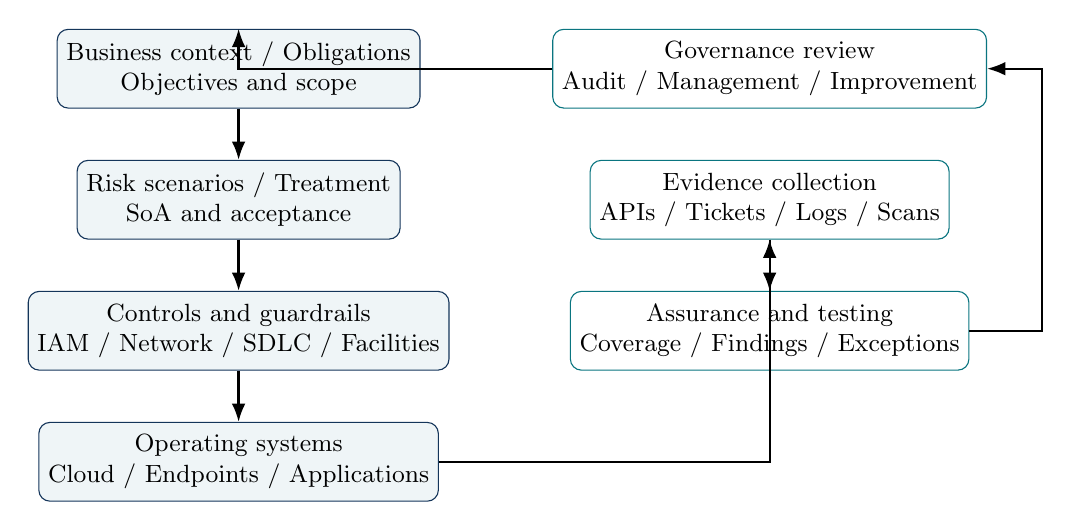
\begin{tikzpicture}[>=Latex,node distance=0.65cm, every node/.style={font=\small},layer/.style={draw=navy,rounded corners,align=center,minimum height=1cm,minimum width=3.7cm,fill=pale},svc/.style={draw=teal,rounded corners,align=center,minimum height=1cm,minimum width=3.7cm,fill=white}]
\node[layer](a){Business context / Obligations\\Objectives and scope};
\node[layer,below=of a](b){Risk scenarios / Treatment\\SoA and acceptance};
\node[layer,below=of b](c){Controls and guardrails\\IAM / Network / SDLC / Facilities};
\node[layer,below=of c](d){Operating systems\\Cloud / Endpoints / Applications};
\node[svc,right=2.4cm of b](e){Evidence collection\\APIs / Tickets / Logs / Scans};
\node[svc,below=of e](f){Assurance and testing\\Coverage / Findings / Exceptions};
\node[svc,above=of e](g){Governance review\\Audit / Management / Improvement};
\draw[->,thick](a)--(b);\draw[->,thick](b)--(c);\draw[->,thick](c)--(d);
\draw[->,thick](d.east)-| (e.south);\draw[->,thick](e)--(f);\draw[->,thick](f.east)-|([xshift=.7cm]g.east)|-(g.east);\draw[->,thick](g.west)-|(a.north);
\end{tikzpicture}}\end{center}
\section{Traceable security architecture decisions}
\small\rowcolors{2}{pale}{white}\begin{longtable}{p{.22\linewidth}p{.36\linewidth}p{.36\linewidth}}
\rowcolor{navy} \textcolor{white}{\textbf{AD record field}} & \textcolor{white}{\textbf{Required engineering question}} & \textcolor{white}{\textbf{Example}}\\
\endfirsthead
\rowcolor{navy} \textcolor{white}{\textbf{AD record field}} & \textcolor{white}{\textbf{Required engineering question}} & \textcolor{white}{\textbf{Example}}\\
\endhead
Context & Which objectives and assets are exposed? & Customer API handling regulated personal data\\
Decision & Which trust boundary or control design is selected? & Service identity with workload federation\\
Alternatives & Which feasible alternatives and drawbacks were evaluated? & Long-lived secret rejected for rotation risk\\
Risk mapping & What risks and control IDs relate? & R-APP-014; 5.16, 8.2, 8.24, 8.27\\
Verification & How is design behavior challenged? & Deny issuance to unauthorized branch/environment\\
Evidence & How will ongoing operation be proven? & Identity grants, deployment logs, signed decisions\\
\end{longtable}\normalsize

\section{Layered security patterns}
\small\rowcolors{2}{pale}{white}\begin{longtable}{p{.20\linewidth}p{.51\linewidth}p{.23\linewidth}}
\rowcolor{navy} \textcolor{white}{\textbf{Layer}} & \textcolor{white}{\textbf{Key decisions}} & \textcolor{white}{\textbf{Representative control references}}\\
\endfirsthead
\rowcolor{navy} \textcolor{white}{\textbf{Layer}} & \textcolor{white}{\textbf{Key decisions}} & \textcolor{white}{\textbf{Representative control references}}\\
\endhead
Organization & Ownership, legal constraints, supplier assurance and incident planning & 5.1, 5.2, 5.19--5.24, 5.31\\
People & Education, remote access responsibilities, termination obligations & 6.1--6.8\\
Physical & Entry, secure locations, media, utilities and disposal & 7.1--7.14\\
Identity and access & Identity lifecycle, elevation, strong authentication, repository rights & 5.15--5.18, 8.2--8.5\\
Data & Classify, minimize, protect and delete information & 5.12--5.14, 8.10--8.12, 8.24\\
Software delivery & Secure design, testing, approved change and environment boundaries & 8.25--8.33\\
Operations & Configuration, vulnerability exposure, logs, monitoring and continuity & 8.8, 8.9, 8.13--8.16\\
\end{longtable}\normalsize

\section{Trust boundary and deployment reviews}
\begin{enumerate}
\item List principals, workloads, stores, trust zones, dependencies and data classification.
\item Draw ingress/egress, human/admin control planes, CI/CD identities and supplier interfaces.
\item Identify inappropriate trust transitions, replay paths, SSRF reachability and excess privileges.
\item Select security requirements and control implementation with owners.
\item Write concrete deny-tests and incident handling behaviors; attach results to decisions.
\item Record accepted gaps with scoped, expiring business-owner approval.
\end{enumerate}

\section{Example architectural acceptance criteria}
\begin{itemize}
\item A non-production identity cannot directly deploy to production; a test demonstrates denial.
\item Production data cannot be downloaded by a developer unless time-bound authorization is recorded.
\item A compromised single service identity cannot enumerate all customer partitions.
\item Every privileged grant creates an append-only observation with reliable timestamp.
\item The restoration design is demonstrated, not assumed, against agreed recovery outcomes.
\end{itemize}

\section{Architecture review pack}
\begin{itemize}
\item Scope and assets inventory with ownership
\item Data flow and trust boundary diagram
\item Threat model with risk traceability
\item Architecture Decision Records (ADRs)
\item Deployment and identity model
\item Control test specification with negative cases
\item Operations, incident and recovery runbooks
\item Approved residual risks and SoA updates
\end{itemize}

\clearpage\section*{Source and interpretation policy}
\addcontentsline{toc}{section}{Source and interpretation policy}
\textbf{Source editions:} ISO/IEC 27000:2018 (overview and vocabulary); ISO/IEC 27001:2022 (requirements and normative Annex A); ISO/IEC 27002:2022 corrected 2022-03 (control guidance). Specific clause identifiers are references to the supplied editions, not reproduced control text.\par
\textbf{Interpretation:} ``Source-grounded paraphrase'' describes a concept in the cited source. ``Engineering recommendation'' is a practical model, technology choice, owner, evidence example, frequency, template or scoring convention authored for this suite; it is not a claim that ISO prescribes that exact approach.\par
\textbf{Conformity:} Clauses 4--10 of ISO/IEC 27001 govern ISMS conformity. Applicability of controls is determined through risk treatment, with Annex A used as a completeness cross-check and exclusions justified in the Statement of Applicability (SoA). Source documents alone neither certify an ISMS nor prove control operating effectiveness.\par
\textbf{Source licensing:} Do not distribute or embed the licensed standard PDFs in repositories or distribute copied normative text. Review the editions, amendments, and certification scheme applicable to each assessment before relying on this work.\par
\end{document}
